\documentclass[preprint]{sigplanconf}

\usepackage{amssymb}
\usepackage{multicol}
\usepackage{xcolor}
\usepackage{graphicx}
\usepackage[fleqn]{amsmath}
\usepackage[hang,flushmargin]{footmisc}
\usepackage{graphics}
\usepackage{stmaryrd}
\usepackage{amsthm}
\usepackage[hyphens]{url}
\usepackage{hyperref}
\usepackage[notquote]{hanging}
\usepackage[T1]{fontenc}
\usepackage{semantic}
\usepackage{enumitem}
\usepackage{flushend}

% =================================================================================================

% TODO: The model here does not actually use type erasure!!
% TODO: Explain why we can only provide simple classes (!)
% TODO: Insert a few more mentions of why "s1 + s2 <: s1 + s2 + s3" is valid (cannot do complete pattern match)

\urlstyle{sf}

\makeatletter
\renewcommand{\@makefntext}[1]{%
  \parindent 1em%
  \raggedright
  \begin{hangparas}{0.8em}{1}
  \noindent {$^{\@thefnmark}$~#1}
  \end{hangparas}
}
\makeatother

\newcommand{\langl}{\begin{picture}(4.5,7)
\put(1.1,2.5){\rotatebox{60}{\line(1,0){5.5}}}
\put(1.1,2.5){\rotatebox{300}{\line(1,0){5.5}}}
\end{picture}}
\newcommand{\rangl}{\begin{picture}(4.5,7)
\put(.9,2.5){\rotatebox{120}{\line(1,0){5.5}}}
\put(.9,2.5){\rotatebox{240}{\line(1,0){5.5}}}
\end{picture}}

\newcommand{\lang}{\begin{picture}(5,7)
\put(1.1,2.5){\rotatebox{45}{\line(1,0){6.0}}}
\put(1.1,2.5){\rotatebox{315}{\line(1,0){6.0}}}
\end{picture}}
\newcommand{\rang}{\begin{picture}(5,7)
\put(.1,2.5){\rotatebox{135}{\line(1,0){6.0}}}
\put(.1,2.5){\rotatebox{225}{\line(1,0){6.0}}}
\end{picture}}

\newcommand{\llangl}{\langl\hspace{-0.35em}\langl}
\newcommand{\rrangl}{\rangl\hspace{-0.35em}\rangl}

\definecolor{cmtclr}{rgb}{0.0,0.6,0.0}
\definecolor{numclr}{rgb}{0.0,0.4,0.0}
\definecolor{kvdclr}{rgb}{0.0,0.0,0.6}
\definecolor{strclr}{rgb}{0.5,0.1,0.0}
\definecolor{prepclr}{rgb}{0.0,0.0,0.0}

\newcommand{\kvd}[1]{\textnormal{\textcolor{kvdclr}{\sffamily #1}}}
\newcommand{\num}[1]{\textnormal{\textcolor{numclr}{\sffamily #1}}}
\newcommand{\str}[1]{\textnormal{\textcolor{strclr}{\sffamily "#1"}}}
\newcommand{\strf}[1]{\textnormal{\textcolor{strclr}{\sffamily #1}}}
\newcommand{\ident}[1]{\textnormal{\sffamily #1}}
\newcommand{\lident}[1]{\textnormal{\sffamily\`{}\hspace{-0.25em}\`{}\hspace{-0.1em}#1\`{}\hspace{-0.25em}\`{}}}
\newcommand{\cmt}[1]{\textit{\sffamily\textcolor{cmtclr}{#1}}}

\newcommand{\lsep}[0]{\;\; | \;\;}
\newcommand{\narrow}[1]{\hspace{-0.85em} #1 \hspace{-0.85em}}

\newcommand{\tsep}[0]{\; \triangledown \;}
\newcommand{\tytag}{\ident{tag}}
\newcommand{\dropopt}[1]{\lfloor#1\rfloor}
\newcommand{\addopt}[1]{\lceil#1\rceil}
\newcommand{\tytagof}{\ident{tagof}}
\newcommand{\nameoftag}{\ident{nameof}}

\newcommand{\reduce}{\rightsquigarrow}

\newcommand{\sem}[1]{\llbracket #1 \rrbracket}
\newcommand{\semalt}[1]{\llangl #1 \rrangl}

\newtheorem{definition}{Definition}
\newtheorem{theorem}{Theorem}
\newtheorem{lemma}{Lemma}

% =================================================================================================

\makeatletter
\def\@copyrightspace{\relax}
\makeatother
\begin{document}

\special{papersize=8.5in,11in}
\setlength{\pdfpageheight}{\paperheight}
\setlength{\pdfpagewidth}{\paperwidth}
\conferenceinfo{CONF 'yy}{Month d--d, 20yy, City, ST, Country}
\copyrightyear{20yy}
\copyrightdata{978-1-nnnn-nnnn-n/yy/mm}
\doi{nnnnnnn.nnnnnnn}

%\titlebanner{Unpublished draft, March 2015}        % These are ignored unless
%\preprintfooter{short description of paper}   % 'preprint' option specified.

\title{F\# Data: \textnormal{Accessing structured data made easy}}
%\subtitle{Subtitle Text, if any}

\authorinfo{Tomas Petricek}
           {University of Cambridge}
           {tomas@tomasp.net}
\maketitle

% =================================================================================================

\section{Introduction}

Programming may not be the new \emph{literacy}, but it is finding its way into many areas
of modern society. For example, making sense of large amounts of data that are increasingly made
available through open government data initiatives\footnote{In the US (\url{http://data.gov}) and
in the UK (\url{http://data.gov.uk}).} is almost impossible without some programming skills.
In media, \emph{data journalism} reflects this development. Data journalists still write articles
and focus on stories, but programming is at the core of their work.

Improving support for data access in programming language can make understanding data simpler,
more usable and reproducible:

\begin{itemize}
  \item \textbf{Simpler.} Many programming languages treat data as foreign entities that have to
    be parsed or processed. Instead, data should be treated as first-class entities fully integrated
    with the rest of the programming language.
  \item \textbf{Usability.} Modern developer tools make coding easier with auto-complete and early
    error checking. Unfortunately, these typically rely on static types which, in turn, make
    programming with standard untyped data harder.
  \item \textbf{Reproducible.} Data journalists often use a wide range of tools (including Excel,
    scripts and other ad-hoc tools). This makes it hard to reproduce the analysis and detect
    errors when the input data changes.
\end{itemize}

\noindent
The presented work reconcilles the \emph{simplicity} of data access in dynamically-typed programming
languages with the \emph{usability} and \emph{reproducibility} provided by statically-typed
languages. More specifically, we develop F\# type providers for accessing data in structured
data formats such as CSV, XML and JSON, which are frequently used by open government data initiatives
as well as other web-based data sources.

% =================================================================================================

\section{Motivation: Accessing structured data}

Despite numerous schematization efforts, most data on the web is available without an explicit
schema. At best, the documentation provides a number of typical requests and sample responses.
For simplicity, we demonstrate the problem using the OpenWeatherMap service, which can be used to get
the current weather for a given city\footnote{See ``Current weather data'': \url{http://openweathermap.org/current}}.
The page documents the URL parameters and shows one sample JSON response to illustrate the
response structure.

\paragraph{Statically-typed.}
In a statically typed functional language like F\#, we could use a library for working with HTTP
and parsing JSON to call the service and read the temperature. Here, the parsing library returns a
value of a \ident{JsonValue} data type and we use pattern matching to extract the value we
need\footnote{We abbreviate the full URL:
\url{http://api.openweathermap.org/data/2.5/weather?q=Prague\&units=metric}}:

\noindent
\begin{equation*}
\begin{array}{l}
 \kvd{let}~\ident{data}=\ident{Http.Request}(\str{http://weather.org/?q=Prague}) \\[0.1em]
 \kvd{match}~\ident{JsonValue.Parse}(\ident{data})~\kvd{with} \\[0.1em]
 |~\ident{Record}(\ident{root})\rightarrow \\[0.1em]
 \quad \kvd{match}~\ident{Map.find}~\str{main}~\ident{root}~\kvd{with} \\[0.1em]
 \quad |~\ident{Record}(\ident{main})\rightarrow \\[0.1em]
 \quad \quad \kvd{match}~\ident{Map.find}~\str{temp}~\ident{main}~\kvd{with} \\[0.1em]
 \quad \quad |~\ident{Number}(\ident{num})\rightarrow \ident{printfn}~\str{Lovely \%f degrees!}~\ident{num} \\[0.1em]
 \quad \quad |~\_\rightarrow \ident{failwith}~\str{Incorrect format} \\[0.1em]
 \quad |~\_\rightarrow \ident{failwith}~\str{Incorrect format} \\[0.1em]
 |~\_\rightarrow \ident{failwith}~\str{Incorrect format}
\end{array}
\end{equation*}
\vspace{0.1em}

\noindent
The pattern matching assumes that the response has a
particular format (as described in the documentation). The root node must be a record with a
\str{main} field, which has to be another record containing a \str{temp} field with a numerical
value. When the format is incorrect, the data access simply fails with an exception.

The code is complicated, because data is parsed into a fully general data structure that we then
process. The code is not benefiting from the generality of the data structure -- quite the opposite!

\paragraph{Dynamically-typed.}
Doing the same in JavaScript is shorter and simpler (not surprisingly, as JSON has been designed
after a subset of JavaScript). Using jQuery to perform the request, we can write:
%
\begin{equation*}
\begin{array}{l}
\ident{jQuery.ajax}(\str{http://weather.org/?q=Prague}, \\
\quad \kvd{function}(\ident{data})~\{ \\
\qquad \kvd{var}~\ident{obj} = \ident{JSON.parse}(\ident{data}); \\
\qquad \ident{write}(\str{Lovely }, \ident{obj.main.temp}, \str{ degrees!}); \\
\quad \});
\end{array}
\end{equation*}
%
Although the code is shorter, writing it is not \emph{easier} than writing the original
statically-typed version. Even though some JavaScript editors provide auto-completion, they
will fail to help us here, because they have no knowledge of the shape of the object \ident{obj}.
So, the author will have to open the documentation and guess the available fields from the
provided sample.

\paragraph{Type providers.}
This paper presents the F\# Data library that implements \emph{type providers} for accessing
structured  data formats such as XML, JSON and CSV. Using the JSON type provider, we can write code
with the same functionality in three lines, but with full editor support including auto-complete
on the \ident{obj} object:
%
\begin{equation*}
\begin{array}{l}
 \kvd{type}~\ident{W} = \ident{JsonProvider}\langl\str{http://weather.org/?q=Prague}\rangl \\
 \kvd{let}~\ident{obj} = \ident{W.GetSample}() \\
 \ident{printfn}~\str{Lovely \%f degrees!}~\ident{obj.main.temp}
\end{array}
\end{equation*}
\vspace{0.0em}

\noindent
On the first line, $\ident{JsonProvider}\langl\str{...}\rangl$ invokes a type provider at
compile-time with the URL as a sample. The type provider infers the structure of the response
from the sample and provides a type that has a statically known property \ident{main}, returning
an object with a property \ident{temp} that provides the temperature as a number.

This gives us the best of both worlds -- the \emph{simplicity} of dynamic typing with the
\emph{usability}, \emph{safety} and associated tooling common in statically-typed languages.

% =================================================================================================

\section{Background: Type providers}

This paper presents a collection of \emph{type providers} for integrating structured data into the
F\# programming language. As outlined in the previous example, our key technical contribution is the
algorithm that infers appropriate type from an example document and and the type providers that
expose the type. In this section, we give a brief overview of the type provider mechanims and of
related approaches to integrating data into programming languages.

\subsection{How type providers work}

Documents in the JSON format consists of several possible kinds of values. The OpenWeatherMap
example in the introduction used only (nested) record and a numerical value. To demonstrate other
aspects, we look at a more complex example that also invloves collections and strings:
%
{\small{
\begin{verbatim}
  [ { "name": "Jan", "age": 25 },
    { "name": "Alexander", "age": 3.5 },
    { "name": "Tomas" } ]
\end{verbatim}
}}
%
\noindent
Say we want to print the names of people in the list with an age if it is available. Assuming
\strf{people.json} contains the above sample and \ident{data} is a string value
that contains another data set in the same format, we can use \ident{JsonProvider} as follows:
%
\begin{equation*}
\begin{array}{l}
 \kvd{type}~\ident{People}~=~\ident{JsonProvider}\langl\str{people.json}\rangl\hspace{1em} \\ [0.6em]
 \kvd{let}~\ident{items}~=~\ident{People.Parse}(\ident{data})\\
 \kvd{for}~\ident{item}~\kvd{in}~\ident{items}~\kvd{do}\\
 \quad\ident{printf}~\str{\%s }~\ident{item.name}\\
 \quad\ident{Option.iter}~(\ident{printf}~\str{(\%f)})~\ident{item.age}
\end{array}
\end{equation*}
%
In contrast to the earlier example, the example now uses a local file \strf{people.json} as a
\emph{representative sample} for the type inference, but then processes data (available at
run-time) from another source.

\paragraph{Type providers.}
The notation $\ident{JsonProvider}\langl\str{people.json}\rangl$ on the first line passes a
\emph{static parameter} to the type provider. Static parameters are resolved at compile-time,
so the file name has to be a constant. The provider analyzes the sample and generates
a type that we name \ident{People}. In F\# editors, the type provider is also executed at
development-time and so the same provided types are used in code completion.

The \ident{JsonProvider} uses a type inference algorithm discussed below and infers the
following types from the sample:
%
\begin{equation*}
\begin{array}{l}
 \kvd{type}~\ident{Entity}~=  \\
 \quad \kvd{member}~\ident{name}~:~\ident{string} \\
 \quad \kvd{member}~\ident{Age}~:~\ident{option}\langl \ident{decimal}\rangl \\[0.6em]
 \kvd{type}~\ident{People}~=  \\
 \quad \kvd{member}~\ident{GetSample}~:~\ident{unit}~\rightarrow~\ident{Entity}[] \\
 \quad \kvd{member}~\ident{Parse}~:~\ident{string}~\rightarrow~\ident{Entity}[] \\
\end{array}
\end{equation*}
%
The type \ident{Entity} represents the person. The field \ident{Name} is available for all
sample values and is inferred as \ident{string}. The field \ident{Age} is marked as optional,
because the value is missing in one sample. The two sample ages are an integer $25$ and a
decimal $3.5$ and so the common inferred type is \ident{decimal}.

The type \ident{People} provides two methods for reading data. \ident{GetSample} returns the
sample used for the inference and \ident{Parse} parses a JSON string containing data in the same
format as the sample. Since the sample JSON is a collection of records, both methods return an
array of \ident{Entity} values.

\paragraph{Erasing type providers.}
At compile-time, F\# type providers use an erasure mechanism similar to Java Generics \cite{java-erasure}.
A type provider generates types and code that should be executed when members are accessed. In compiled
code, the types are erased and the program directly executes the generated code.
In the above example, the compiled (and actually executed) code looks as follows:

\noindent
\begin{equation*}
\begin{array}{l}
 \kvd{let}~\ident{items}~=~\ident{asArray}(\ident{JsonValue.Parse}(\ident{data}))\\
 \kvd{for}~\ident{item}~\kvd{in}~\ident{items}~\kvd{do}\\
 \quad\ident{printf}~\str{\%s }~\ident{asString}~(\ident{getProp}~\str{name}~\ident{item})\\
 \quad\ident{Option.iter}~(\ident{printf}~\str{(\%f)})\\
 \qquad(\ident{Option.map}~\ident{asFloat}~(\ident{tryGetProp}~\str{age}~\ident{item}))
\end{array}
\end{equation*}
%
The generated type \ident{Entity} is erased to a type $\ident{JsonValue}$, which represents any
JSON value and is returned by the \ident{Parse} method. The remaining properties are erased to
calls to various operations of the type provider runtime such as \ident{asArray}, \ident{getProp}
or \ident{asFloat} that attempt to convert a JSON value into the required structure (and produce
a run-time exception if this is not possible).

The (hidden) type erasure process turns the static provided types into code that we might write
without type providers. In particular, checked member names become unchecked strings. A type
provider cannot remove all possibilities for a failure -- indeed, an exception still occurs if the
input does not have the right format, but it simplifies writing code and removes most errors when
a representative sample is provided.

\subsection{Type systems and data integration}
The F\# Data library connects two lines of research that have been previously disconnected. The
first is extending the type systems of programming languages and the second is inferring the
structure of real-world data sources.

The type provider mechanism has been introduced in F\# \cite{fsharp-typeprov,fsharp-typeprov-ddfp}
and used in areas such as semantic web \cite{liteq}. The library presented in this paper is the
most widely used library of type providers and it is also novel in that it shows the programming
language theory behind a concrete type provider.

\paragraph{Extending the type systems.}
A number of systems integrate external data formats into a programming language. Those include
XML \cite{xduce,xduce-ml} and databases \cite{links}. In both of these, the system either requires
the user to explicitly define the schema (using the host language) or it has an ad-hoc extension
that reads the schema (\emph{e.g.}~from a database). LINQ \cite{linq} is more general, but relies
on code generation when importing the schema.

The work that is most similar to F\# Data is the XML and SQL integration in C$\omega$ \cite{comega-xs}.
It extends C\# with types capable of representing structured data formats, but it does not infer
the types from samples and it modifies the C\# language (rather than using a general purpose
embedding mechanism).

Aside from type providers, a number of other advanced type system features could be used to
tackle the problem discussed in this paper. The Ur \cite{ur} language has a rich system for working
with records; meta-programming \cite{template-hask}, \cite{th-camlp4} and multi-stage programming
\cite{multi-stage} could be used to generate code for the provided types. However, as far as we
are aware, none of these systems have been used to provide the same level of integration with
XML, CSV and JSON.

\paragraph{Typing real-world data.}
The second line of research related to our work focuses on inferring structure of real-world data sets.
A recent work on JSON \cite{typing-json} infers a succinct type using MapReduce to handle large number
of samples. It fuses similar types based on a type similarity measure. This is more sophisticated than
our technique, but it would make formally specifying the safety properties difficult.

The PADS project \cite{pads-dsl,pads-ml} tackles a more general problem of handling \emph{any} data format.
The schema definitions in PADS are similar to our structural type. The structure inference for LearnPADS
\cite{pads-learn} infers the data format from a flat input stream. A PADS type provider could follow
many of the patterns we explore in our work, but formally specifying the safety property would be
again challenging.

% =================================================================================================

\section{Approach and uniqueness}

The F\# Data library relies on two key techniques. First, it implements a type inference algorithm
that generates a suitable type from one or more sample documents. Second, it implements a type
provider that turns this \emph{structural type} into an ordinary F\# type that is then used by
the programmers. The mapping preserves an important property that we call \emph{relativized type
safety}. Informally, we prove that when the provided sample is \emph{representative}, code written
using the type provider will not fail.

Whether a sample is \emph{representative} is formally described using a subtyping relation
on structural types $\sigma$. The full definition of the relationship can be found in our recent
report \cite{fsharp-data-paper}. In this paper, we provide a brief overview and discuss one
interesting case in detail.

\subsection{Structural types}
\label{sec:inference-types}

The grammar below defines a \emph{structural type} $\sigma$. We distinguish between \emph{non-nullable types}
that always have a valid value (written as $\hat{\sigma}$) and \emph{nullable types} that encompass missing
and \kvd{null} values (written as $\sigma$). We write $\nu$ for record field:
%
\begin{equation*}
\begin{array}{rcl}
 \hat{\sigma} &\narrow{=}& \{ \nu_1 : \sigma_1, \ldots, \nu_n : \sigma_n \} \\[0.1em]
              &\narrow{|}& \ident{float} \lsep \ident{int} \lsep \ident{bool} \lsep \ident{string}
 \\[0.6em]
       \sigma &\narrow{=}& ~\hat{\sigma}~ \lsep \hat{\sigma}\;\,\kvd{option} \lsep [\sigma] \\[0.1em]
              &\narrow{|}& \sigma_1 + \ldots + \sigma_n \lsep ~\top~ \lsep \kvd{null}
\end{array}
\end{equation*}
%
The non-nullable types include records (consisting of zero or more fields with their types) and
primitive types (\ident{int} for integers, \ident{float} for floating-point numbers, strings and
Booleans).

Any non-nullable type is also a nullable type, but it can be wrapped in the \kvd{option}
constructor to explicitly permit the \kvd{null} value. These are typically mapped to the standard
F\# option type. A simple collection type $[\sigma]$ is also nullable and missing values or
\kvd{null} are treated as empty collection. The type $\kvd{null}$ is inhabited by the $\kvd{null}$
value (using an overloaded but not ambiguous notation) and $\top$ represents the top type.

Finally, a union type in our model implicitly permits the \kvd{null} value. This is because the
type provided for unions requires the user to handle the situation when none of the case matches
(and so developers always provide code-path that can be run when the value is missing).

% --------------------------------------------------------------------------------------------------

\subsection{Subtyping relation}
\label{sec:inference-subtyping}

The subtyping relation between structural types is illustrated in Figure~\ref{fig:subtyping-diagram}.
We split the diagram in two parts. The upper part shows non-nullable types (with records and
primitive types). The lower part shows nullable types with \kvd{null}, collections and optional
values. We omit links between the two part, but any type $\hat{\sigma}$ is a subtype of
$\hat{\sigma}~\kvd{option}$ (in the diagram, we abbreviate $\sigma~\kvd{option}$ as $\sigma?$).
The following excerpt specifies some of the relationships formally:

\begin{definition}
$\sigma_1 :> \sigma_2$ denote that $\sigma_2$ is a subtype of $\sigma_1$. The
subtyping relation is defined as a transitive reflexive closure of:

\begin{align}
\ident{float}\,:>\,\ident{int}\\[-0.2em]
\sigma :> \kvd{null} \quad &(\textnormal{iff}~\sigma \neq \hat{\sigma}) \\[-0.2em]
\hat{\sigma}~\kvd{option} :> \hat{\sigma} \quad &(\textnormal{for all}~\hat{\sigma})
\end{align}
\begin{align}
 \{ \nu_1\!:\!\sigma_1, .., \nu_n\!:\!\sigma_n \} &:>  \{ \nu_1\!:\!\sigma_1', .., \nu_n\!:\!\sigma_n' \}
   \;\,\quad (\sigma_i \hspace{-0.25em}:>\hspace{-0.25em} \sigma_i') \\
 \{ \nu_1\!:\!\sigma_1, .., \nu_n\!:\!\sigma_n \} &:>  \{ \nu_1\!:\!\sigma_1, .., \nu_m\!:\!\sigma_m \}
   \quad (m \hspace{-0.1em}\geq\hspace{-0.1em} n) \\
 \{ \nu_1\!:\!\sigma_1, .., \nu_n\!:\!\sigma_n \} &:> \{ \nu_{\pi(1)}\!:\!\sigma_{\pi(1)}, .., \nu_{\pi(m)}\!:\!\sigma_{\pi(m)} \}
\end{align}
\vspace{-1.5em}
\begin{align}
\hspace{-0.6em}
\begin{array}{l}
 \{ \nu_1\!:\!\sigma_1, .., \nu_n\!:\!\sigma_n, \nu_{n+1}\!:\!\kvd{null}, .., \nu_{n+m}\!:\!\kvd{null} \} :> \\
 \{ \nu_1\!:\!\sigma_1, .., \nu_n\!:\!\sigma_n \}
\end{array}
\end{align}
\end{definition}

% --------------------------------------------------------------------------------------------------

\begin{figure}
\begin{center}
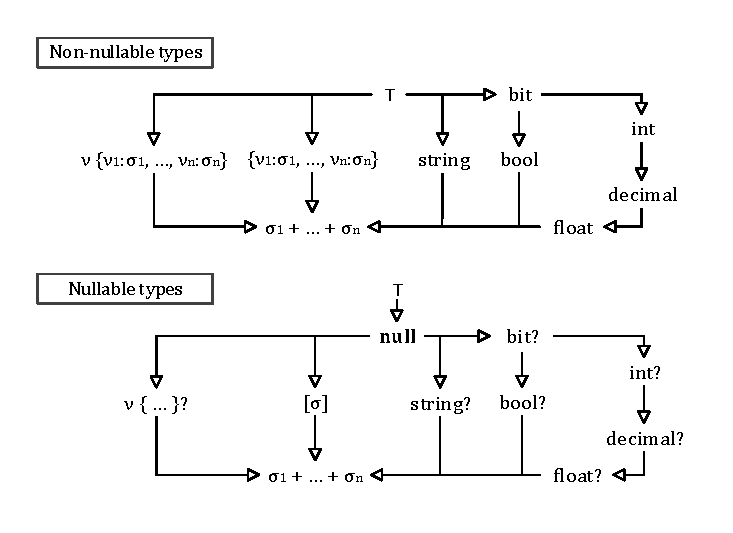
\includegraphics[scale=0.75,trim=5mm 5mm 5mm 5mm,clip]{images/hierarchy.pdf} % left bottom right top
\end{center}
\vspace{-0.5em}
\caption{Subtype relation between structural types}
\label{fig:subtyping-diagram}
\vspace{-0.5em}
\end{figure}

% -------------------------------------------------------------------------------------------------
\noindent
Here is a summary of the key aspects of the definition:

\begin{itemize}
\item For numeric types (1), we infer the most precise numeric type that can represent all values
  from a sample dataset (even though this means loss of precision in some cases).

\item The \kvd{null} type is a subtype of all nullable types (2), that is all
  $\sigma$ types excluding non-nullable types $\hat{\sigma}$). Any non-nullable type is also a
  subtype of its optional version (2).

\item The subtyping on records is covariant (4), subtype can have
  additional fields (5) and fields can  be reordered (6). The interesting rule
  is (7) -- together with covariance, it states that a subtype can omit some
  fields, provided that their types are nullable.
\end{itemize}

\noindent
The rule that allows subtype to have fewer record elements (8) is particularly
important. It allows us to prefer records in some cases. For example, given two samples
$\{ \ident{name}:\ident{string} \}$ and $\{ \ident{name}:\ident{string}, \ident{age}:\ident{int} \}$,
we can find a common supertype $\{ \ident{name}:\ident{string}, \ident{age}:\ident{int}~\kvd{option} \}$
which is also a record. For usability reasons, we prefer this to another common supertype
$\{ \ident{name}:\ident{string} \} + \{ \ident{name}:\ident{string}, \ident{age}:\ident{int} \}$.
Working with records does not require pattern matching and it makes it easier to explore data
in editors that provide auto-completion.

% -------------------------------------------------------------------------------------------------

\begin{figure*}[t]
\noindent
\begin{equation*}
\hspace{3em}
\inference[(record)\;]
  { (\nu_i = \nu'_j \Leftrightarrow (i = j) \wedge (i \leq k))
      \qquad \forall i\in\{ 1 .. k \}.(\sigma_i \tsep \sigma'_i \vdash \sigma''_i) }
  { \begin{array}{l}
    \{ \nu_1 : \sigma_1,  \; \ldots \;, \nu_k : \sigma_k, \; \ldots \;, \nu_n : \tau_n \} \tsep
    \{ \nu'_1 : \sigma'_1, \; \ldots \;, \nu'_k : \sigma'_k, \; \ldots \;, \nu'_m : \tau'_m \} \vdash\\
    \{ \nu_1 : \sigma''_1, \; \ldots \; , \nu_k : \sigma''_k,
                            \nu_{k+1} : \addopt{\sigma_{k+1}}, \ldots, \nu_n : \addopt{\sigma_n},
                            \nu'_{k+1} : \addopt{\sigma'_{k+1}}, \ldots, \nu'_m : \addopt{\sigma'_m} \}
    \end{array} }
\end{equation*}

\begin{equation*}
\hspace{3em}
% collection types
\inference[(list)\;]
  {\sigma_1 \tsep \sigma_2 \vdash \sigma}
  {[\sigma_1] \tsep [\sigma_2] \vdash [\sigma]}
\qquad
% primitive types
\inference[(prim)\;]
  { }
  {\ident{int} \tsep \ident{float} \vdash \ident{float}}\quad
\qquad
% null and nullable
 \begin{array}{l}
 \textnormal{\footnotesize{(null-1)}}\;\; \sigma \tsep \kvd{null} \vdash \sigma \quad(\sigma :> \kvd{null}) \\[0.6em]
 \textnormal{\footnotesize{(null-2)}}\;\; \sigma \tsep \kvd{null} \vdash \sigma~\kvd{option} \quad(\sigma :\ngtr \kvd{null})
 \end{array}
\end{equation*}

\caption{Selected inference judgements that define the common supertype relation}
\label{fig:subtyping-cst}
\end{figure*}

% --------------------------------------------------------------------------------------------------


\subsection{Common supertype relation}
\label{sec:inference-commonsuper}

As demonstrated by the example in the last section, structured types do not have a unique greatest
lower bound. Our inference algorithm prefers records over unions and is defined in terms of the
\emph{common supertype} relation. The type infernce obtains a type for each sample (or each element
of a collection) and then uses the relation to finds their common type. To demonstrate the idea,
we show the definition for primitive types and records:

\begin{definition}
A \emph{common supertype} of types $\sigma_1$ and $\sigma_2$ is a type $\sigma$, written
$\sigma_1 \triangledown \sigma_2 \vdash \sigma$, obtained according to the inference rules in
Figure~\ref{fig:subtyping-cst} (remaining rules can be found in the report \cite{fsharp-data-paper}).
\end{definition}

\noindent
When finding a common supertype of two records (\emph{record}), we return a record type that has the union
of fields of the two arguments. We assume that the names of the first $k$ fields are the same and the
remaining fields have different names (other rules permit reordering of fields). The types of shared
fields become common supertypes of their respective types (recursively). Fields that are present in
only one record are marked as optional using the following helper definition:

\begin{equation*}
\begin{array}{rcll}
 \addopt{\hat{\sigma}} &\narrow{=}& \hat{\sigma}~\kvd{option} \qquad&(\textnormal{non-nullable types})\\
 \addopt{\sigma} &\narrow{=}& \sigma &(\textnormal{otherwise})
\end{array}
\end{equation*}

\noindent
Discussing the full system is out of the scope of this paper, but the system has a number of desirable
properties -- the common supertype is uniquely defined and it is a supertype of both of the
provided examples. Furthermore (to aid usability) our algorithm finds a common supertype that is not
a union, if such type exists.

% =================================================================================================

\section{Results and contribution}

The contributions and results of the presented work fall in three categories. First, our work is
interesting in that it looks at a concrete type provider from the perspective of programming language
theory and we introduce a novel notion of \emph{relativized type safety}. Second, the F\# Data library
has become the most frequently downloaded F\# library and is de-facto standard for data access in F\#.
Third, the work is also interesting from philosophical perspective because it illustrates an important
change in thinking about types that we need to adopt when developing types for systems in the
modern age of the web.

\subsection{Relativized type safety}

The safety property of F\# Data type providers states that, given representative sample documents,
any code that can be written using the provided types is guaranteed to work. We call this
\emph{relativized safety}, because we cannot avoid \emph{all} errors. In particular, the user can
always use the type provider with an input that has a different structure than any of the samples --
and in this case, it is expected that the code will fail at runtime. Our formal model
\cite{fsharp-data-paper} states precisely what inputs can be handled by a provided type:
%
\begin{itemize}[noitemsep]
\item[--] Input can contain smaller numerical values (for example, if a sample contains float, the input can contain an integer).
\item[--] Records in the actual input can have additional fields.
\item[--] Records in the actual input can have fewer fields, provided that the type of the fields is marked as optional in the sample.
\item[--] Union types in the input can have both fewer or more cases.
\item[--] When we have a union type in the sample, the actual input can contain values of any of the union cases.
\end{itemize}
%
This is proved by our safety theorem, which relies on a simplified model of type providers and the
F\# language. We follow the approach of syntactic type safety \cite{syntactic} and show the type
preservation (reducing expression does not change type) and progress (an expression that is not a
value can be reduced).

\begin{theorem}[Relativized safety]
\label{thm:safety}
Assume $s_1, \ldots, s_n$ are samples, $\sigma$ is a common supertype of the types of $s_i$.
Next, assume that the type provider maps structural type $\sigma$ to an F\# type $\tau$ and that
it provides a function $f$ that takes an input $s$ and produces a value $\tau$.

Then for all new inputs $s'$ that are subtypes of one of the samples $s_i$, and for any expression
$e_c$ (user code) such that $x:\tau \vdash e_c:\tau'$, it is the case that
$e_c[x\leftarrow f(s')] \rightarrow^{*} v$ for value $v$ and $\vdash v:\tau'$.
\end{theorem}

\subsection{New perspective on static typing}

The \emph{relativized safety} property does not guarantee the same amount of safety as standard
type safety for programming languages without type providers. However, it reflects the reality of
programming with external data sources that is increasingly important in the age of the web.
In short, type providers do not \emph{reduce} the safety -- they simply \emph{reveal} an existing issue.

In a separate paper \cite{age-of-web}, we argue that this is an important futrue direction for
programming languages. Programs increasingly access external data sources (be it open government
data accessed by data journalists or services consumed by mobile applications). Most programming
language theory treats programs as closed expressions with no external dependencies -- this gives
us a formally tractable model, but it ``throws out the baby with the bath water''. Our experience
with F\# Data suggests that we can accept the reality of working with data \emph{and} still
provide clear formal model with provable safety properties.

\subsection{Practical experience}

The F\# Data library has become the standard library for accessing data in F\# and is widely used
by both open-source projects and commercial users of F\#. At the time of writing, it has 38
contributors and it has over 43,000 downloads\footnote{The first version (providing the functionality
discussed here) has been created by the author of this paper; further contributions added new features
and significantly improved the portability and overall quality of the library.
See \url{https://github.com/fsharp/FSharp.Data}.}.

The success of the library provides an evidence that some of the pragmatic (and perhaps
controversial) choices made in the F\# Data design work well in practice:

\begin{itemize}
\item The fact that a provided type may fail at run-time is not a problem as developers expect this
  when working with external data. In practice, the input that caused the issue can be added as
  another sample -- the new compilation errors show which part of the program need to be modified
  to handle the input correctly.

\item The F\# Data library has been designed to work well with modern F\# editors that use the
  F\# compiler to provide auto-completion based on static types\footnote{This includes Visual
  Studio, Emacs, Xamarin Studio, Atom and others.}. The success of F\# Data confirms that editting
  experience and interactive development are important aspect of modern programming environments.
\end{itemize}


% =================================================================================================

\section{Conclusions}

The F\# Data library presented in this paper simplifies working with structured data formats such
as XML, JSON and CSV. This is achieved by using the type provider mechanism to integrate external
structured data into the programming language. We briefly outlined the programming language theory
behind F\# Data as well as its practical usability properties that contributed to its adoption.

Accessing and processing data is becoming an important ability in the modern information-rich
society and we believe that tools such as F\# Data can make programming simpler, more usable
and more trustworthy -- and, for example, enable data journalists produce analyses that their
readers can not just understand, but also verify and modify.

\bibliographystyle{plain}
\bibliography{paper}


\end{document}
